\documentclass{article}
\usepackage{tikz}
\usetikzlibrary{shapes.geometric, arrows.meta, positioning}
\begin{document}
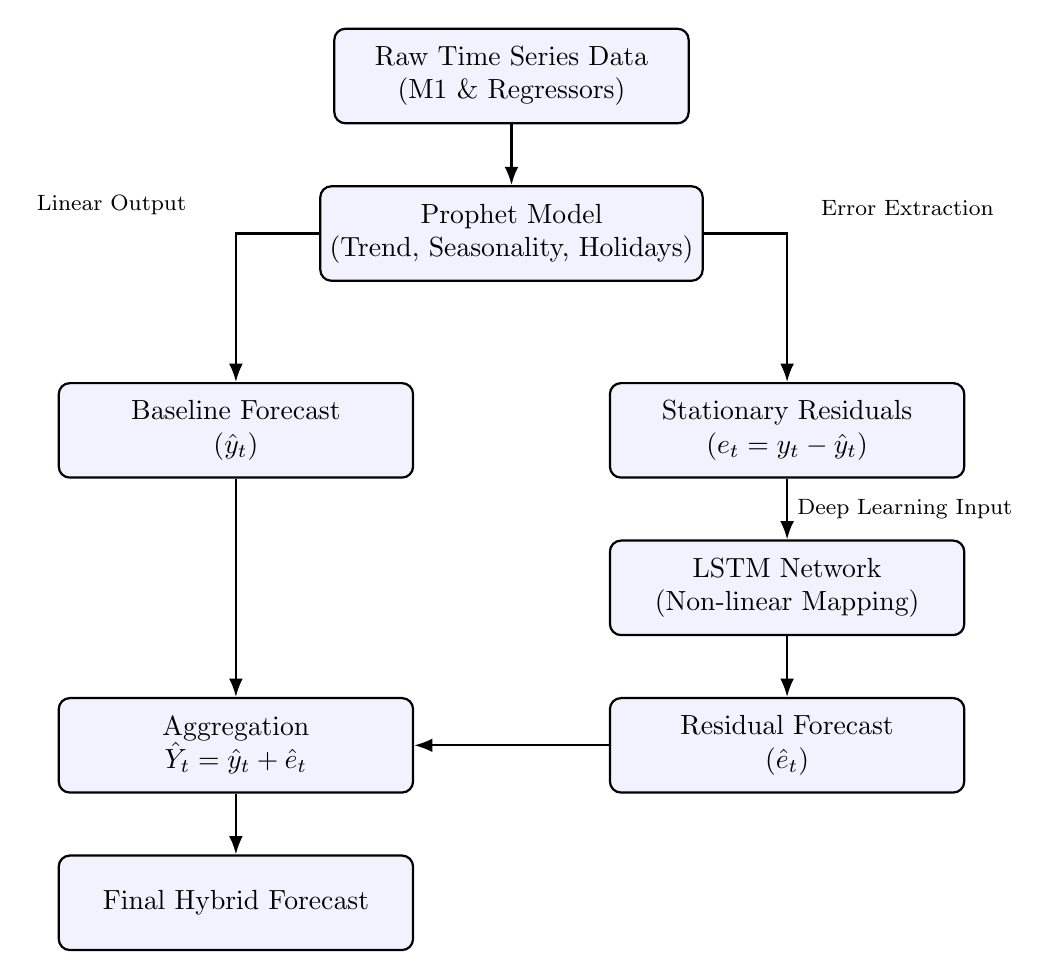
\begin{tikzpicture}[
    box/.style={rectangle, draw, thick, align=center, minimum width=4.5cm, minimum height=1.2cm, fill=blue!5, rounded corners},
    arrow/.style={-Latex, thick}
]

% Nodes using absolute positioning for exact control
\node[box] (input) at (0, 0) {Raw Time Series Data \\ (M1 \& Regressors)};
\node[box] (prophet) at (0, -2) {Prophet Model \\ (Trend, Seasonality, Holidays)};
\node[box] (baseline) at (-3.5, -4.5) {Baseline Forecast \\ ($\hat{y}_t$)};
\node[box] (residuals) at (3.5, -4.5) {Stationary Residuals \\ ($e_t = y_t - \hat{y}_t$)};
\node[box] (lstm) at (3.5, -6.5) {LSTM Network \\ (Non-linear Mapping)};
\node[box] (lstm_pred) at (3.5, -8.5) {Residual Forecast \\ ($\hat{e}_t$)};
\node[box] (combine) at (-3.5, -8.5) {Aggregation \\ $\hat{Y}_t = \hat{y}_t + \hat{e}_t$};
\node[box] (final) at (-3.5, -10.5) {Final Hybrid Forecast};

% Arrows
\draw[arrow] (input) -- (prophet);
\draw[arrow] (prophet) -| node[above left=0.1cm and 0.5cm, font=\footnotesize] {Linear Output} (baseline);
\draw[arrow] (prophet) -| node[above right=0.1cm and 0.3cm, font=\footnotesize] {Error Extraction} (residuals);
\draw[arrow] (residuals) -- node[right, font=\footnotesize] {Deep Learning Input} (lstm);
\draw[arrow] (lstm) -- (lstm_pred);
\draw[arrow] (baseline) -- (combine);
\draw[arrow] (lstm_pred) -- (combine);
\draw[arrow] (combine) -- (final);

\end{tikzpicture}
\end{document}
